% Chapter 3

\chapter{Modelisation de l'EDP en 2D} % 3rd chapter title

\label{Chapter3} % For referencing the chapter elsewhere, use \ref{Chapter3} 

%----------------------------------------------------------------------------------------

Ayant resolu le modele en 1D durant le stage, on procede dans cette partie a sa modelisation en 2D. Il s'agit de resoudre le probleme direct du transfer radiatif avant de passer au probleme inverse dans la partie suivante. On rappelle breivement le modele considere avant de decrite l'implementation que utilisee.

\section{Le transfert radiatif}


On considère un rayonnement transporté par des particules de masse nulle appelés photons. Lorsqu'ils se touvent en presence de la matiere, les photons inteassgissent avec celle. Trois phonomees sont preponderant (\ref{Fig:TranfertRadiatif}):

\begin{itemize}
 \item l'emission: Les photons sont emis en reponse aux electrons excites descendants a des niveaux d'energie plus bas. Ce phenomenes est caraterise par l'opacite d'émission $\sigma_e$. Il s'agit de l'inverse du libre parcours d'emision \footnote{Le libre par cours moyen d'emission represente la distance moyenne entre deux emissions de photons. Les libres parcours d'absorption et de dispersion sont definis de maniere similaire}. Plus la temperature matiere est elevee, plus ce phenomene est important.
 \item l'absorption: A l'inverse, certains photons sont absorbes par la matiere. Ce pehenomene se caraterise par l'opacite d'absorption $\sigma_a$. Lorsqu'on est a l'equilibre thermique, $\sigma_e = \sigma_e$.
 \item la dispersion (ou "scaterring" ou parfois diffusion): Certains photons sont devies de leur trajectoire par la matiere. Ce phenomme se caraterise non seulement par son opacite de scatering $\sigma_c$ \footnote{ $\sigma_a$ et $\sigma_c$ sont definis de maniere similaire a $\sigma_e$}, mais aussi par une fonction de distribution angulaire decrivant la maniere dont les photons sont devies.
\end{itemize}

(IMAGE DU TRANFER RADIATIF)

L'equation du transfer radiatif (1) represente un bilan d'energie lie au rayonnement au niveau microscopique. Nous nous placerons dans le cas particulier d'equilibre thermodynamique local (ETL)\footnote{etat dans lequel on peut definir une temperature pour chaque point du domaine, et l'emission est decrite par la fonction de Planck \parencite{Reference3}}. L'equilibre radiatif \footnote{il se produit si la matiere est a l'equilibre avec le reyonnement. Si on est dans l'ETL, les photons sont emis suivant la fonction de Planck a la temperature de la matiere} quant a lui sera considere comme condition initiale pour les simulations.

(EQUATION 1) - ETR (et definition des termes)

Il est possible de modeliser l'ETR a travers plusieurs modeles. Le modele P1 est un modele macroscopique \footnote{ils ne prennent en compte que les varaibles d'espace et de temps et spm obtenu par integration des termes microscopique tels que I par rapport a la frequence et la direction} aux moments (d'ordre 2), lineaire et hyperbolique. Vu que l'energie du rayonnement n'est pas convervee durant sont interaction avec la matiere, il faut coupler le modele P1 avec une equation regissant l'energie de la matiere. On utilisera une equation d'energie amtiere simplifiee qui ne tient compte que des termes d'echange avec le rayonnement. Le modele P1 couple a la matiere (REF FRACNK) est presente ci-bas:

(EQUATION 2) - MODELE P1  E, F, et T)

Comme on peut le voir a travers la definition de $E$ et $F$, notre modele est dit "gris" car nous l'integrons sur tout le spectre de frequence. En effet, nous ne nous interressons qu'au rayonnement a travers son bilan d'energie transporte par le flux radiatif. Sur ce point, la version du modele P1 que nous avons utilise est mois precise qu'un modele microscopique base soit sur une methode Monte-Carlo ou une methode des ordonnes discrete. Neanmoins notre modele presente l'avantage d'etre tres peu couteux et relativement facile a implementer \parencite{Reference3}. 
%----------------------------------------------------------------------------------------

\section{Schéma de splitting}

Le modele P1 tend vers une equation de diffusion lorsque les opcites d'absorption ($sigma_a$) et de dispersion ($sigma_c$) sont elevees (de facon a ce que $c/sigma_a = 1$). Les schema classiques tels que le schema de Rusanov ne sont pas assez precis pour capturer cette propriete. 

(EQ 3 - LIMITE DE FISSUSION)

Le schema en 2 etape (ou de Splitting) propose par (franck) est assez precis pour traduire la limite de diffusion. Les deux etapes sont resumees co-bas.


\subsection{Etape 1}
La premiere etape (dite etape de couplage ou d'equilibre, ou etape de relaxation de la temperature) permet de regler la temperature sur chaque maille (independament des autres mailles). On ne considere que les equations ou la temperature est impiquee (equations 1 et 3 du modele p1), en fixant la valeur du flux sur chaque maille. Il s'agit d'une methode de point fixe qui est toujorus definie. \parencite{Reference2}

Le domaine rectangulaire est suppose discretise en $N \times M$ mailles uniformes. $j$ denote l'identifiant d'une cellule (Figure \ref{fig:2DMesh}).

(SCHEMA DE SPLiTTING - etape 1)

On itere sur q jusq'a ce que E et $\Theta$ convergent vers $E^*$ et $\Theta^*$.

\subsection{Etape 2}
Il s'agit ici de resoudre les deux EDP hyperboliques en 1 et 2. 
Avasnt d'qttquer le schema schema de splitting, on note que les equations 1 et 2 du modele P1 sont hyperboliques et que La methode des volumes finis est donc adaptee pour les resoudre.

(VOLUMES FINIS)

Nous retournons donc sur le maillage disretise en definisant les different flux numeriques impliques. Durant cette etape, il faut considerer l'ajout de mailles fantommes, ce qui porte le nombre total de volumes a $(N+2) \times (M+2)$.

\begin{figure}[H]
\begin{subfigure}{.6\textwidth}
  \centering
  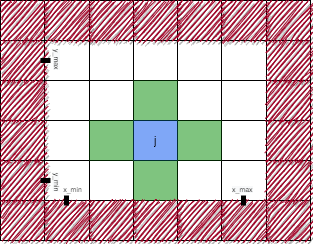
\includegraphics[width=.8\linewidth]{Dicretisation2D}  
  \caption{Dicretisation du domaine}
  \label{fig:Discretisation2D}
\end{subfigure}
\begin{subfigure}{.4\textwidth}
  \centering
  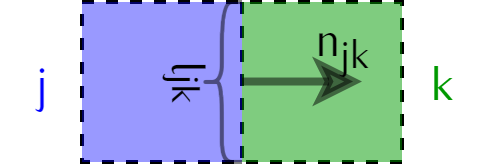
\includegraphics[width=.8\linewidth]{Interaction2D}  
  \caption{Interaction entre deux mailles j et k}
  \label{fig:Interaction2D}
\end{subfigure}
\caption{Dicretisation du maillage 2D. Sur la figure (A), on peut observer les mailles dites "fantomes" hachurees en rouge. Les quatre maille voisine d'une maille j sont indiquees en vert. Le volume de la maille j est definie par $\Omega_j$. Le nombre de mailles suivant l'rizontale $M$ est choisi telle que le maillage soir uniforme i.e $\Delta x = \frac{x_{max}-x_{min}}{N} = \frac{y_{max}-y_{min}}{M} = \Delta y$. Sur la figure (B), on observe la defintion de la normale sortante $n_{jk}$ de la mailles j. On peut aussi observer la longeur caracteristique $l_{jk}$}
\label{fig:2DMesh}
\end{figure}

(SCHEMA DE SPLiTTING etape 2) (\parencite{Reference4})

%----------------------------------------------------------------------------------------

\section{Implementation en C++}

Le dode de calcul a ete develope durant la 4 eme semaine du stage. Etant donne des parametre du probleme, il permet d'exporter les signaux temporels $E, F \text{et} T$ sur les quatres bords du domaine. Pour raisons de visualisation, il permet aussi dd'exporter les signaux sur l'entierete du domaine en tout temps. Ces signaux peuvent ensuite etre visualiser sous forme d'une animation a l'aide d'un notebook construit a cet effet.

L'executable se nomme \verb|transfer| et est disponible avec le reste du code sur le repository Github \href{https://github.com/desmond-rn/projet-inverse-2d}{projet-inverse-2d}.

\subsection{Configuration du modele}

L'executable necessite un fichier de Configuration pour s'excuter. Les parametres a definir sont indiques ci-dessous.

(RAPPELLER L'ASPECT D'UN FICHIER CONFIG)

Un exemple de fichier de configuration pourrait se predenter comme ceci:

(IMAGE DF SIMU)


\subsection{Sauvegarde des données}

Comme mentione ci-haut, on dispose de deux options pour sauvegarder les resultats de la simulation:

\begin{itemize}
 \item sous le forme CSV: Ce mode permet une visualisation facile des resultats a l'aide du noteook. Il est tres couteux en espace memoire et necessite la Librairie Pandas pour le lire en forme de dataframe. Cette operation prend une quantite non negligeagle de RAM, ce qui peut nuire a l'usage qu'on veut faire des donnes.
 
 \item sous le format SDS \footnote{source-densite-signal}: Ce format binaire ne sauvegarde que les informations les plus importante de la simualtion. En locurence la source utilisee, la densite du domaine, et les diffetents signaux sur les bords du domaine. Il est particulieremtnt interressant pour generer les donnees necessaires a l'apprentissage. Les details concernatn la ce format sont donnes en annexe \ref{AppendixA}.
\end{itemize}

%----------------------------------------------------------------------------------------

\section{Résultats}

Queslques resultats obtenus sont presentes ici. Les images ci-bas sont obtenus avec le fichier de configuration (IMAGE DF SIMU). La source est une onde sinusoidale placee en $E$ sur la gauche. La densitee en particulier a la forme d'un signal en crenau egale a 0.1 en dehors du crenau et a 10 en dehors. Les opacites d'absorbes sont proportionelles a la densite.

(ENERGIE ET FLUX OBSTACLE CIRCULAIRE - au temps final)

On peut observer une asorption presque totale du signal au niveau du crenau du a la forte valeur des opacite d'absorption et d'emission. En ce sens, le saut de densite agit comme un obstacle a la propagation du signal. l'evolution de l'energie et du flux sur les bords du domaine traduit l'effet qu'a la densite sur la propagation du signal. Sur les images, la cause du probleme direct (la densite) est affichee au centre des figures, et les effets sont presentes aux alentours.

(EVOLUTION SUR LES BORDS)

Nous testons ensuite notre modele sur le cas tres particulier de la limite de diffusion, un attout important du schema de splitting que nous avons implemente. Dans ce cas, les opacites en dehors de l'obstacle sont de l'ordre de $c$. Le bord gauche est continuement chauffe et l'obstacle est un crenau ayany la forme d;un rectangle vu du haut. (On se sert des lignes de niveau pour observer les variations du signal avec plus de precisions)

(ENERGIE ET FLUX OBSTACLE RECTANGULAIRE - LIMITE DE DIFFUSION)

(EVOLUTION SUR LES BORDS)

On confirme effectiment l'effet de diffusion du signal dans le domaine. Nous pouvons a present passer au probleme inverse proprement dit. 

%----------------------------------------------------------------------------------------
